\subsection{Koordinatsystem}
\label{Koordinatsystem}

Det koordinatsystem som brukar användas i Matematik 2B är tvådimensionellt och består av två reella tallinjer som är vinkelräta och möter varann i \textit{origo} där båda är $0$.

En position, eller \textit{koordinat}, i koordinatsystemet anges som $(x, y)$ där $x$ anger positionen längs den horisontella \textit{x-axeln} och $y$ anger positionen längs den vertikala \textit{y-axeln}.

Här är ett exempel på en koordinat $A = (3, 1)$ i detta koordinatsystem:

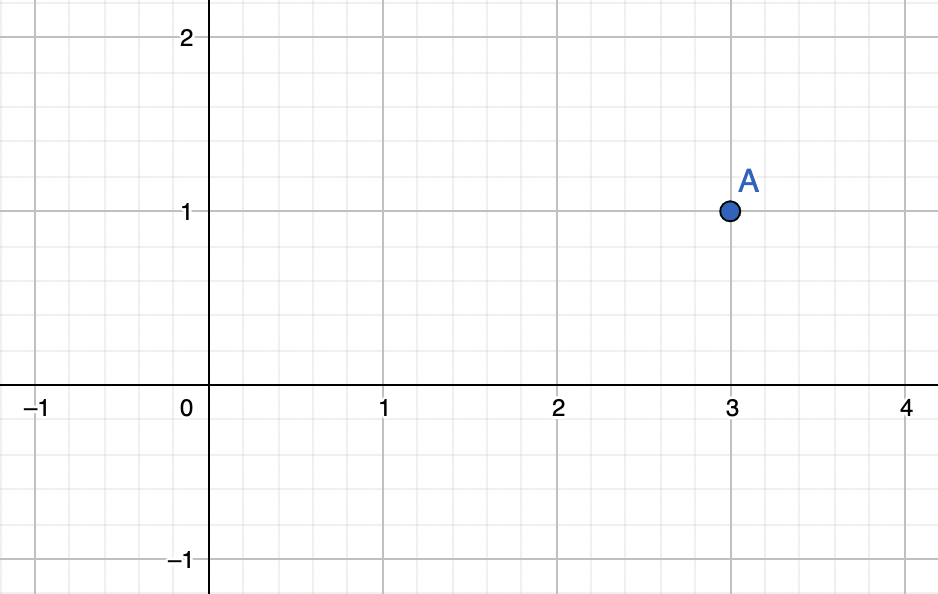
\includegraphics[width=\textwidth]{img/1.png}

\subsection{Funktion}

En funktion inom Matematik 2B är något som översätter ett nummer till ett annat. Ett exempel är denna funktion $f$,

\begin{align}
	f(x) = \frac{1}{2}x-1
\end{align}

som översätter $2$ till $0$, eller $4$ till $1$.

vi kan rita up $f$ grafiskt i koordinatsystemet från \ref{Koordinatsystem}, genom att låta $f(x) = y$.

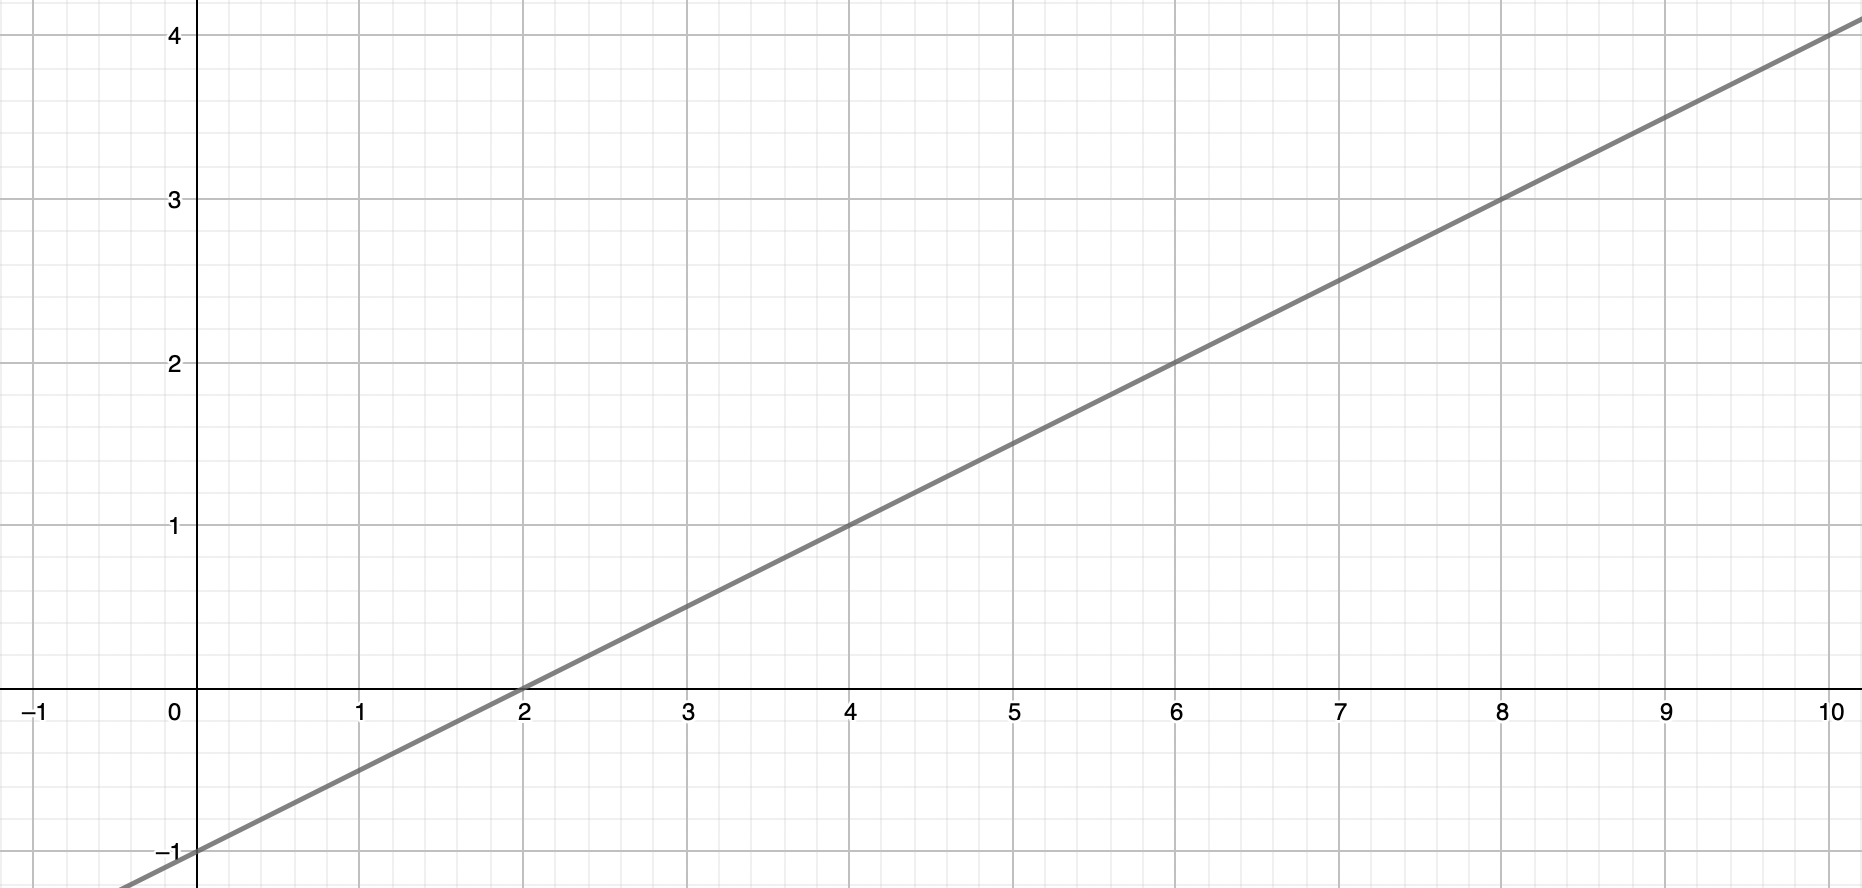
\includegraphics[width=\textwidth]{img/2.png}